\documentclass{article}

\usepackage[dblblindworkshop]{neurips_2026}

\usepackage[utf8]{inputenc}
\usepackage[T1]{fontenc}
\usepackage{hyperref}
\usepackage{url}
\usepackage{booktabs}
\usepackage{amsfonts}
\usepackage{nicefrac}
\usepackage{microtype}
\usepackage{xcolor}
\usepackage{graphicx}

\title{Compression Breaks Discipline: Quantization Increases Missed Tool Calls\\in Small Language Models, but Not Mid-Size Ones}

\author{
  Anonymous authors\\
  Paper under double-blind review
}

\begin{document}

\maketitle

\begin{abstract}
Small language models are increasingly deployed as tool-calling agents under
tight memory budgets, where 4-bit post-training quantization (NF4) is the
standard compression choice. Prior evaluations of quantized models report
aggregate accuracy, which can hide \emph{which kinds} of failures change even
when the overall score appears stable. We audit the error distribution of
tool-calling behavior under quantization using a seven-class error taxonomy
over 600 controlled generations from two Qwen3 models (1.7B and 4B), each
tested at FP16 and NF4 on Berkeley Function Calling Leaderboard single-turn
tasks with identical greedy decoding. Our central finding is a size-dependent
behavioral shift: for Qwen3-1.7B, NF4 nearly triples missed required tool
calls (6.0\% to 17.3\%; $\Delta=-11.3$pp, bootstrap 95\% CI $[-19.3,-4.7]$),
spread across all task categories; for Qwen3-4B the same comparison shows no
effect (7.3\% vs.\ 7.3\%, CI $[-6.0,+6.0]$) with nominally higher accuracy.
Aggregate accuracy moves by only a few points in both cases and would not
reveal this asymmetry. These results suggest that (i) quantization damage in
agents manifests primarily as a loss of tool-calling \emph{discipline} rather
than knowledge, and (ii) safe 4-bit deployment thresholds are model-size
dependent. We release our taxonomy classifier, generation protocol, and
per-answer labels to support error-profile audits beyond scalar accuracy.
\end{abstract}

\section{Introduction}
\label{sec:intro}

Tool-calling language models power a growing share of applied agent systems:
they translate user requests into structured calls against APIs, databases,
and calculators~\citep{schick2023toolformer,yao2023react}. In deployment,
these models are frequently compressed to 4-bit weights via post-training
quantization to fit consumer GPUs and edge budgets; NF4 in particular is the
default format behind popular inference stacks~\citep{dettmers2023qlora}.
The implicit assumption is that quantization is a benign, near-lossless
operation: benchmark accuracy typically drops by only a point or two.

This paper asks whether that assumption survives when we stop looking at one
number per model and instead look at the \emph{distribution of failure
types}. A model whose accuracy holds at 75\% but which silently stops calling
required tools is a very different production risk than one that occasionally
mis-formats arguments---yet both look identical under aggregate scoring.

We study this question with a controlled experiment. Two Qwen3 instruction
models (1.7B and 4B)~\citep{yang2025qwen3} answer single-turn
Berkeley Function Calling Leaderboard (BFCL)
tasks~\citep{yan2024bfcl} at FP16 and at 4-bit NF4, with decoding held
exactly constant across formats (greedy, temperature 0, fixed seed, thinking
disabled). Every response is labeled with a seven-class error taxonomy that
separates behavioral failure modes: missing a required call, calling an
unnecessary tool, choosing the wrong tool, supplying wrong arguments,
malformed output, failed execution, and truncation.

Our main result is an asymmetric, size-dependent shift. For the 1.7B model,
NF4 raises missed-required-call errors from 6.0\% to 17.3\%
($\Delta=-11.3$pp, 95\% CI $[-19.3,-4.7]$); the increase appears across all
five task categories rather than concentrating in one. The same comparison in
the 4B model shows no detectable shift (CI $[-6.0,+6.0]$) and nominally
\emph{higher} accuracy under NF4. Meanwhile overall accuracy moves by fewer
than eight points everywhere---within ranges commonly reported as
``quantization is fine.''

Our contributions are:
\begin{itemize}
  \item A pre-registered, controlled protocol for auditing quantization via
  error-taxonomy shifts, holding tokenizer, chat template, sampling, and
  parser fixed across formats (\S\ref{sec:method}).
  \item Evidence that 4-bit quantization degrades tool-calling discipline in
  small (1.7B) but not mid-size (4B) models, invisible to accuracy-only
  reporting (\S\ref{sec:results}).
  \item A practical implication: memory-saving quantization decisions for
  agent deployments should be validated per model size against
  behavioral---not just scalar---metrics.
\end{itemize}

We deliberately scope claims to what was measured: one model family, one
quantization method, single-turn tasks. \S\ref{sec:limitations} states these
boundaries explicitly.

\section{Related Work}
\label{sec:related}

\textbf{Quantization of LLMs.} Post-training quantization research has
largely been evaluated by perplexity and downstream task
accuracy~\citep{dettmers2022llmint8,frantar2023gptq,lin2024awq,xiao2023smoothquant,gholami2022survey}.
NF4~\citep{dettmers2023qlora} is widely used because it retains quality at 4
bits. This literature rarely reports \emph{failure-mode distributions};
our work complements it by asking not ``how much accuracy is lost'' but
``which behaviors break.''

\textbf{Tool use and agentic evaluation.} Benchmarks such as BFCL, AgentBench,
and $\tau$-bench score agents on end-to-end tool-calling
success~\citep{yan2024bfcl,liu2023agentbench,yao2024taubench}. BFCL's own
analyses examine error categories, but quantization studies built on such
suites typically publish only aggregate pass rates. We reuse BFCL tasks and
ground truth while applying our own taxonomy layer, so that the audit does
not depend on any particular leaderboard's internal checker.

\textbf{Function-calling model families.} Gorilla and successors established
fine-tuned API-calling models~\citep{patil2023gorilla}; modern instruction
models such as Qwen3 ship native tool-call formats. We study exactly this
native-format regime, since deployed agents consume these structured outputs.

\section{Method}
\label{sec:method}

\subsection{Design overview}

We compare each model to itself across quantization formats, eliminating all
non-quantization variance: identical prompts, tools, tokenizer, chat
template, greedy decoding (temperature 0, seed fixed, thinking mode
disabled), maximum new tokens (192), and parsing logic. The only difference
between arms is weight precision: FP16 versus NF4 (4-bit, double-quantized,
FP16 compute dtype) via bitsandbytes 0.50.1 with transformers 5.0.0. All
generation ran on NVIDIA T4 GPUs; every version pin, prompt file hash, and
seed is recorded in our artifact metadata.

\subsection{Tasks and data}

We use BFCL v4 single-turn categories covering complementary capability
axes: \texttt{simple\_python} (single required call), \texttt{parallel}
(multiple simultaneous calls), \texttt{multiple} (multiple sequential
requests), and the \texttt{live\_*} variants collected from real user
queries. From each category we take the first 30 entries, yielding $n=150$
responses per model--format cell, 600 total. The sample size was fixed in a
pre-registration written before the run, together with the decision rule
used in \S\ref{sec:results}; no design element changed after data collection.

\subsection{Error taxonomy}

Each response is parsed with a format-independent extractor for the Qwen3
native tool-call syntax and assigned exactly one label:

\begin{enumerate}
  \item \textbf{missed required call}: the ground truth requires a call; none occurs;
  \item \textbf{unnecessary call}: a call is made where none is warranted;
  \item \textbf{wrong tool}: a different tool is called than required;
  \item \textbf{right tool, wrong args}: correct tool, incorrect or missing arguments;
  \item \textbf{malformed}: output unparseable as a function call;
  \item \textbf{valid output, failed execution}: parses but would fail at runtime;
  \item \textbf{truncation}: generation cut off by the token budget.
\end{enumerate}

Responses meeting the ground truth are labeled \emph{correct}. The same
classifier runs on every arm, so any systematic parsing bias affects all
cells equally. We additionally log latency, throughput, peak GPU memory, and
output lengths per response.

\subsection{Statistics}

For each class we report proportions with percentile bootstrap confidence
intervals (2{,}000 resamples). Format differences use an independent
two-sample bootstrap on $\Delta = p_{\mathrm{fp16}} - p_{\mathrm{nf4}}$ per
model; a difference is treated as solid when its 95\% CI excludes zero. Our
pre-registered primary endpoint was the missed-required-call difference.

\section{Results}
\label{sec:results}

\begin{figure}[t]
  \centering
  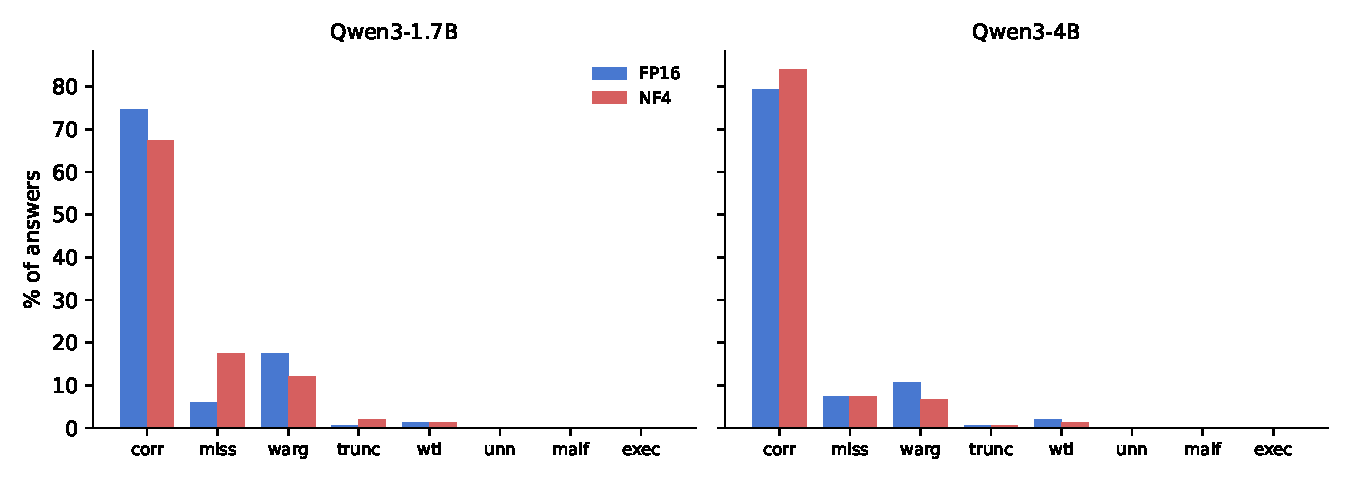
\includegraphics[width=\linewidth]{figures/error_distribution.pdf}
  \caption{Error-type distribution per model and format ($n=150$/cell).
  Most mass sits in \emph{correct}, \emph{wrong-args}, and
  \emph{missed-required}. Only the 1.7B model shows a large NF4-induced
  redistribution, driven almost entirely by missed required calls.}
  \label{fig:dist}
\end{figure}

\begin{table}[t]
\caption{Missed required calls (pre-registered primary endpoint).
$\Delta = p_{\mathrm{fp16}} - p_{\mathrm{nf4}}$ in percentage points;
CIs are independent two-sample bootstrap 95\% intervals.}
\label{tab:main}
\centering
\begin{tabular}{lcccccc}
\toprule
Model & FP16 & NF4 & $\Delta$ & 95\% CI of $\Delta$ & CI excl.\ 0? \\
\midrule
Qwen3-1.7B & 9/150 (6.0\%) & 26/150 (17.3\%) & $-11.3$ & $[-19.3,\,-4.7]$ & Yes \\
Qwen3-4B   & 11/150 (7.3\%) & 11/150 (7.3\%) & $+0.0$  & $[-6.0,\,+6.0]$  & No  \\
\bottomrule
\end{tabular}
\end{table}

\begin{figure}[t]
  \centering
  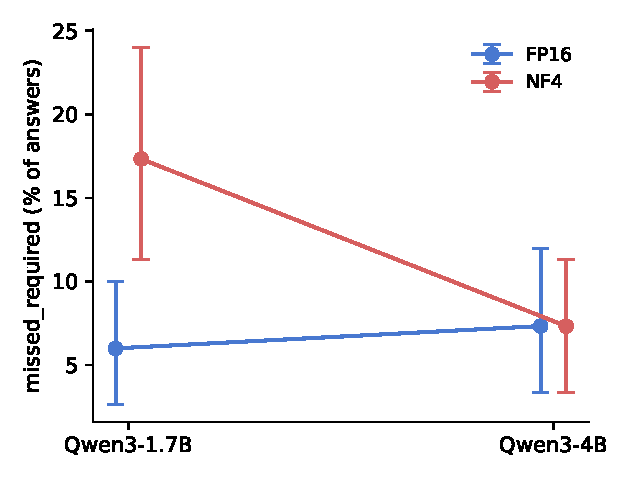
\includegraphics[width=0.55\linewidth]{figures/interaction_missed_required.pdf}
  \caption{Size $\times$ format interaction on missed required calls
  (means with bootstrap 95\% CIs). The quantization effect is present only
  at 1.7B.}
  \label{fig:interaction}
\end{figure}

\textbf{A solid, replicated-magnitude shift in the 1.7B model.}
Under NF4, missed required calls rise from 6.0\% to 17.3\%---a roughly
threefold rate increase whose difference CI excludes zero comfortably
(Table~\ref{tab:main}). This confirms the direction observed in a smaller
n=50 pilot (2\% vs.\ 12\%) with a tighter interval. The effect is not an
artifact of one category: NF4 misses appear in all five BFCL categories
(4/3/3/8/8 misses per category) whereas FP16 misses concentrated in the
live-user subsets (0/0/0/2/7).

\textbf{No effect---and nominally better accuracy---in the 4B model.}
The same protocol detects nothing at 4B: eleven missed calls in each arm
(CI $[-6.0,+6.0]$, bounding any true effect to within about six points).
If anything, NF4 slightly improves this model (accuracy 84.0\% vs.\ 79.3\%;
wrong-args 6.7\% vs.\ 10.7\%), consistent with reports that mild noise can
regularize larger networks.

\textbf{Accuracy alone hides the story.}
Across cells, aggregate correctness spans only 67--84\% and its format
differences have CIs crossing zero in both models. A practitioner reading
only accuracy would conclude ``NF4 costs a couple of points'' for both
models. The taxonomy reveals instead that the 1.7B loses a specific,
deployment-relevant capability---remembering to act through tools---while
the 4B is essentially untouched.

\textbf{Cost profile.} NF4 reduced peak GPU memory for the 4B from 7.8GB to
5.9GB ($\sim$25\%), with throughput of 11--18 tok/s on T4 across all cells.
For the 1.7B, those savings come bundled with the discipline degradation
above; for the 4B they appear free under our audit.

\section{Discussion}
\label{sec:discussion}

\textbf{Discipline, not knowledge.} Manual inspection of missed-call cases
shows the quantized 1.7B often produces the correct answer as plain text
(e.g., computing circumference directly) instead of emitting the required
structured call. The capability exists; the behavioral contract weakens.
This distinguishes quantization harm in agents from ordinary capability
loss and explains why scalar benchmarks understate the risk.

\textbf{Why smaller models may be more fragile.} One plausible mechanism is
that adherence to a strict output format is a sharper, more easily perturbed
feature in low-capacity networks, so 4-bit noise tips marginal generations
across the format boundary more often. Our design cannot isolate mechanism;
we flag it for future work with logit-level instrumentation.

\textbf{Practical guidance.} Teams compressing small open models into agents
should run a behavioral audit before deploying NF4 checkpoints: our results
suggest ``does it still call required tools?'' is the first-order question,
ahead of accuracy deltas. At 4B scale, the same audit showed no cost,
indicating that safe compression thresholds are size dependent rather than
universal.

\section{Limitations}
\label{sec:limitations}

Our claims are bounded by design. We study one model family (Qwen3) at two
sizes; other families may differ. We test one quantizer (NF4); GPTQ or AWQ
may behave differently~\citep{frantar2023gptq,lin2024awq}. Tasks are
single-turn; multi-turn and execution-in-the-loop settings may shift or
amplify effects (our taxonomy's failed-execution class requires runtime state
we do not exercise here). $n{=}150$ per cell powers the pre-registered
endpoint but leaves rare classes (e.g., truncation) underpowered. Finally,
the taxonomy is our own instrument; although it is format-independent and
identical across arms, absolute class boundaries involve judgment calls that
other groups may draw differently. The 4B null should be read as ``no
detectable effect within $\pm$6pp,'' not proof of exact equivalence.

\section{Reproducibility statement}

All generation used pinned software (transformers 5.0.0, bitsandbytes 0.50.1,
torch 2.10.0+cu128, Python 3.12.13), a pinned BFCL commit, fixed seeds, and
greedy decoding; prompts are verbatim BFCL v4 files. The classifier, runner
code, pre-registration text, per-answer labels, and machine-readable result
files accompany this paper as supplementary material, alongside plain-text
summaries of every table and figure. Total compute: four T4 GPU-hours.

\bibliography{references}
\bibliographystyle{plainnat}

\appendix

\section{Full per-class results}
\label{app:full}

\begin{table}[h]
\caption{Complete taxonomy breakdown, percent of responses ($n=150$/cell).}
\centering
\small
\begin{tabular}{lcccc}
\toprule
Class & 1.7B FP16 & 1.7B NF4 & 4B FP16 & 4B NF4 \\
\midrule
correct            & 74.7 & 67.3 & 79.3 & 84.0 \\
missed required    & 6.0  & 17.3 & 7.3  & 7.3  \\
wrong args         & 17.3 & 12.0 & 10.7 & 6.7  \\
wrong tool         & 1.3  & 1.3  & 2.0  & 1.3  \\
unnecessary        & 0.0  & 0.0  & 0.0  & 0.0  \\
malformed          & 0.0  & 0.0  & 0.0  & 0.0  \\
failed execution   & 0.0  & 0.0  & 0.0  & 0.0  \\
truncation         & 0.7  & 2.0  & 0.7  & 0.7  \\
\bottomrule
\end{tabular}
\end{table}

Per-category counts of missed required calls under NF4 for Qwen3-1.7B:
simple\_python 4, parallel 3, multiple 3, live-simple 8, live-multiple 8
(FP16: 0, 0, 0, 2, 7), demonstrating category-wide rather than localized
degradation.

\end{document}
